\documentclass[12pt]{article}
\usepackage[margin=1in]{geometry}
\usepackage{amsmath,amsthm,amssymb}

\usepackage[T1]{fontenc}
\usepackage{bigfoot} % to allow verbatim in footnote
\usepackage[numbered,framed]{matlab-prettifier}
\usepackage{filecontents}
\usepackage{graphicx}
\usepackage[normalem]{ulem}

\let\ph\mlplaceholder % shorter macro
\lstMakeShortInline"

\lstset{
  style              = Matlab-editor,
  basicstyle         = \mlttfamily,
  escapechar         = ",
  mlshowsectionrules = true,
}

\title{MAE 275 - Homework 3}
\author{John Karasinski}

\begin{document}
\maketitle

\section{Defining the System}
The longitudinal linearized aircraft equations of motion can be expressed in state space form, with state variables $\Delta u, \Delta w, \Delta q, \Delta \theta, \Delta h $, as
% \begin{equation}
% \begin{split}
% \Delta \dot{u} = &X_u \Delta u + X_w \Delta w - g\cos \theta_0 \Delta \theta + \sum\limits_{i=1}^n X_{\delta_i} \Delta \delta_i \\
% \Delta \dot{w} = &\dfrac{Z_u}{1-Z_{\dot{w}}} \Delta u +
%                   \dfrac{Z_w}{1-Z_{\dot{w}}} \Delta w +
%                   \dfrac{Z_q + u_0}{1-Z_{\dot{w}}} \Delta q -
%                   \dfrac{g\sin \theta_0}{1-Z_{\dot{w}}} \Delta \theta +
%                   \dfrac{1}{1-Z_{\dot{w}}} \sum\limits_{i=1}^n Z_{\delta_i} \Delta \delta_i \\
% \Delta \dot{q} = &\left[ M_u + \dfrac{M_{\dot{w}} Z_u}{1-Z_{\dot{w}}} \Delta u  \right] +
%                   \left[ M_w + \dfrac{M_{\dot{w}} Z_w}{1-Z_{\dot{w}}} \Delta w  \right] +
%                   \left[ M_q + \dfrac{M_{\dot{w}} (Z_q + u_0)}{1-Z_{\dot{w}}} \Delta q  \right] \\
%                  & - \left[ \dfrac{M_{\dot{w}} g\sin \theta_0}{1-Z_{\dot{w}}} \Delta \theta  \right]
%                    + \dfrac{M_{\dot{w}}}{1-Z_{\dot{w}}} \sum\limits_{i=1}^n Z_{\delta_i} \Delta \delta_i
%                    + \sum\limits_{i=1}^n M_{\delta_i} \Delta \delta_i \\
% \Delta \dot{\theta} = &\Delta q \\
% \Delta \dot{h} = &-\Delta w + u_0 \Delta \theta \\
% \end{split}
% \label{long}
% \end{equation}

\begin{equation*}
A =
\begin{bmatrix}
    X_u & X_w & 0 & -g \cos(\theta_0) & 0 \\
    \dfrac{Z_u}{1-Z_{\dot{w}}} & \dfrac{Z_w}{1-Z_{\dot{w}}} & \dfrac{Z_q + u_0}{1-Z_{\dot{w}}} & \dfrac{g\sin \theta_0}{1-Z_{\dot{w}}} & 0 \\
    M_u + \dfrac{M_{\dot{w}} Z_u}{1-Z_{\dot{w}}} & M_w + \dfrac{M_{\dot{w}} Z_w}{1-Z_{\dot{w}}} & M_q + \dfrac{M_{\dot{w}} (Z_q + u_0)}{1-Z_{\dot{w}}} & -\dfrac{M_{\dot{w}} g\sin \theta_0}{1-Z_{\dot{w}}} & 0 \\
    0 & 0 & 1 & 0 & 0 \\
    0 & -1 & 0 & u_0 & 0
\end{bmatrix}
\end{equation*}

\noindent Plugging in the data for the VZ-4 ``Doak'' aircraft in Appendix A of "Aircraft Dynamics and Automatic Control" yields
\begin{equation*}
A =
\begin{bmatrix}
  -1.3700e-1 &          0 &          0 & -3.2200e+1 &           0 \\
           0 & -1.3700e-1 &          0 &          0 &           0 \\
  +1.3600e-2 &          0 & -4.5200e-2 &          0 &           0 \\
           0 &          0 & 1         &          0 &           0 \\
           0 & -1         &          0 &          0 &           0 \\
\end{bmatrix}
\end{equation*}

\noindent Matrices B, C, and D can also be formed
\begin{equation*}
B =
\begin{bmatrix}
   X_{\delta_e} \\
   \dfrac{Z_{\delta_e}}{1-Z_{\dot{w}}} \\
   \dfrac{M_{\dot{w}} Z_{\delta_e}}{1-Z_{\dot{w}}} + M_{\delta_e} \\
   0 \\
   0 \\
\end{bmatrix}
=
\begin{bmatrix}
            0 \\
         1.08 \\
         1.00 \\
            0 \\
            0 \\
\end{bmatrix}
\end{equation*}

\begin{equation*}
C =
\begin{bmatrix}
      % 1 & 0 & 0 & 0 & 0 \\
      % 0 & 1 & 0 & 0 & 0 \\
      % 0 & 0 & 1 & 0 & 0 \\
      % 0 & 0 & 0 & 1 & 0 \\
      % 0 & 0 & 0 & 0 & 1 \\
 0 &    0 &    1 &    1 &    0 \\
\end{bmatrix}
\end{equation*}

\begin{equation*}
D =
\begin{bmatrix}
      % 0 \\
      % 0 \\
      % 0 \\
      % 0 \\
      % 0 \\
 0 \\
\end{bmatrix}
\end{equation*}

\clearpage
\section{System Properties}

\noindent We can find the resulting transfer functions, $\dfrac{q}{\delta e} (s)$ and $\dfrac{\theta}{\delta e} (s)$, with the following commands \\

\begin{filecontents*}{code.m}
C = eye(5);
D = [0; 0; 0; 0; 0];

[n, d] = ss2tf(A, B, C, D);
minreal(zpk(tf(n(3, :),d))) % q
minreal(zpk(tf(n(4, :),d))) % theta
\end{filecontents*}
\lstinputlisting[]{code.m}

\noindent which results in
\begin{filecontents*}{code.m}
              s (s+0.137)
  -----------------------------------
  (s+0.8223) (s^2 - 0.6401s + 0.5326)
\end{filecontents*}
\lstinputlisting[]{code.m}
and
\begin{filecontents*}{code.m}
               (s+0.137)
  -----------------------------------
  (s+0.8223) (s^2 - 0.6401s + 0.5326)
 
\end{filecontents*}
\lstinputlisting[]{code.m}

\noindent The following MATLAB command is called to identify the characteristic roots and eigenvector elements
\begin{filecontents*}{code.m}
[v, d] = eig(A);
\end{filecontents*}
\lstinputlisting[]{code.m}

\noindent resulting in two real eigenvalues and a complex pair of eigenvalues
\begin{equation*}
\begin{split}
d_1 =& -8.2230e-01 \\
d_2 =& -1.3700e-01 \\
d_3 =& +3.2005e-01 \pm i 6.5583e-1 \\
\end{split}
\end{equation*}

\noindent and their associated eigenvectors
\begin{equation*}
\begin{split}
v_1 = [  -9.9962e-1, & \\  
         +0.0000e+0, & \\  
         +1.7494e-2, & \\  
         -2.1275e-2, & \\  
         +0.0000e+0]&,  \\ 
v_2 = [  +0.0000e+0, & \\
         +1.3573e-1, & \\
         +0.0000e+0, & \\
         +0.0000e+0, & \\
         +9.9075e-1]&, \\
v_3 = [  +9.9953e-1, & \\ 
         +0.0000e+0, & \\ 
         +8.8107e-3  & \mp i 1.5820e-2, \\ 
         -1.4187e-2  & \mp i 2.0358e-2, \\ 
         +0.0000e+0  &]  \\ 
\end{split}
\end{equation*}

\clearpage
\section{Designing the Controller}

The transfer function of the system, $VZ-4$, was identified as
\begin{filecontents*}{code.m}
            (s+1) (s+0.137)
  -----------------------------------
  (s+0.8223) (s^2 - 0.6401s + 0.5326)
\end{filecontents*}
\lstinputlisting[]{code.m}

A controller, $G_C$ was designed as
\begin{filecontents*}{code.m}
  10000 (s+0.8223) (s+0.7)^3
  ---------------------------
  s^2 (s+500) (s+1) (s+0.137)
\end{filecontents*}
\lstinputlisting[]{code.m}

\noindent This controller was determined using loop-shaping priciples such that:

The closed-loop system is stable

The $G_C$ has more poles than zeros

The closed-loop bandwidth (-3dB criterion) is at least 5 rad/sec (23.5 rad/sec)

\sout{The gain margin is at least 6dB} (-24 dB)

The phase margin is at least 40 deg (80 deg)

There is zero steady-state error to a step input $\theta_C$


\begin{figure}[h]
\begin{center}
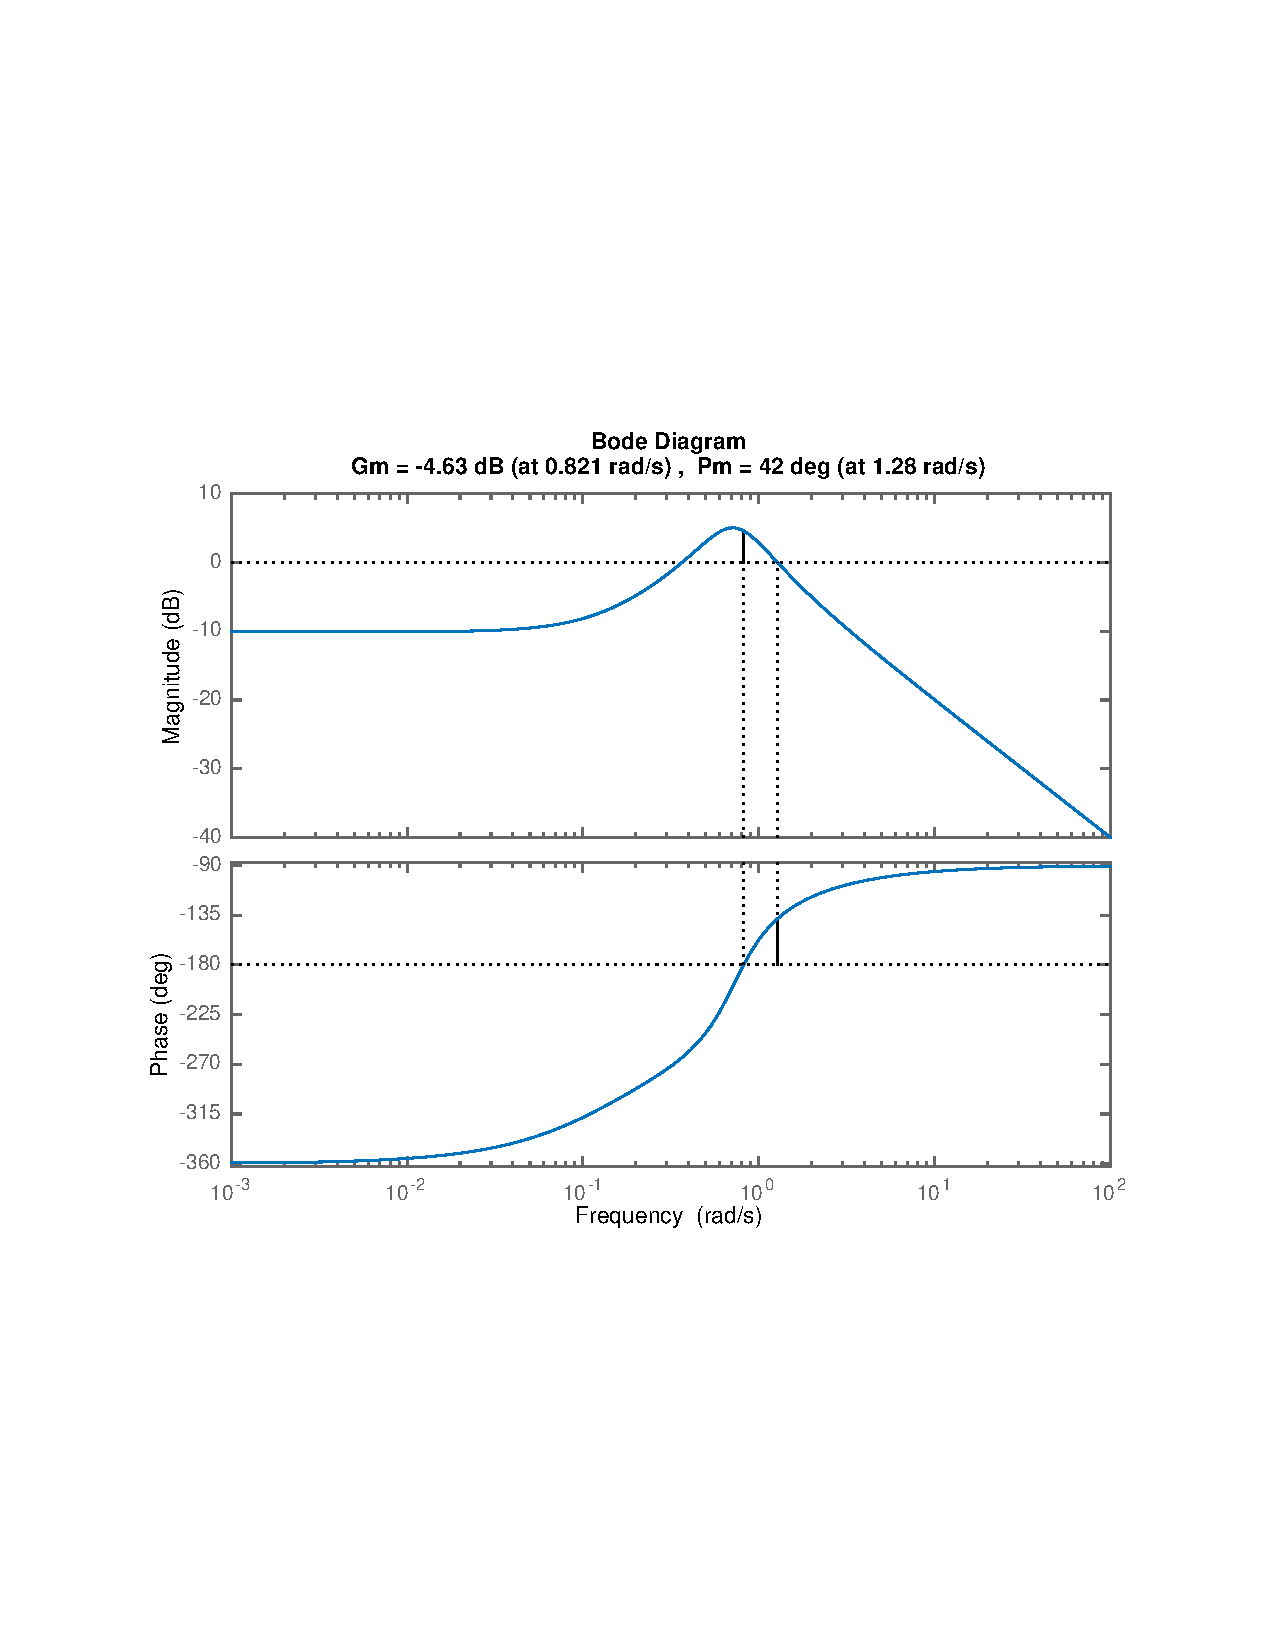
\includegraphics[width=1\textwidth]{figures/open_loop_bode}
\caption{Open Loop Bode Diagram}
% \label{}
\end{center}
\end{figure}

\begin{figure}[h]
\begin{center}
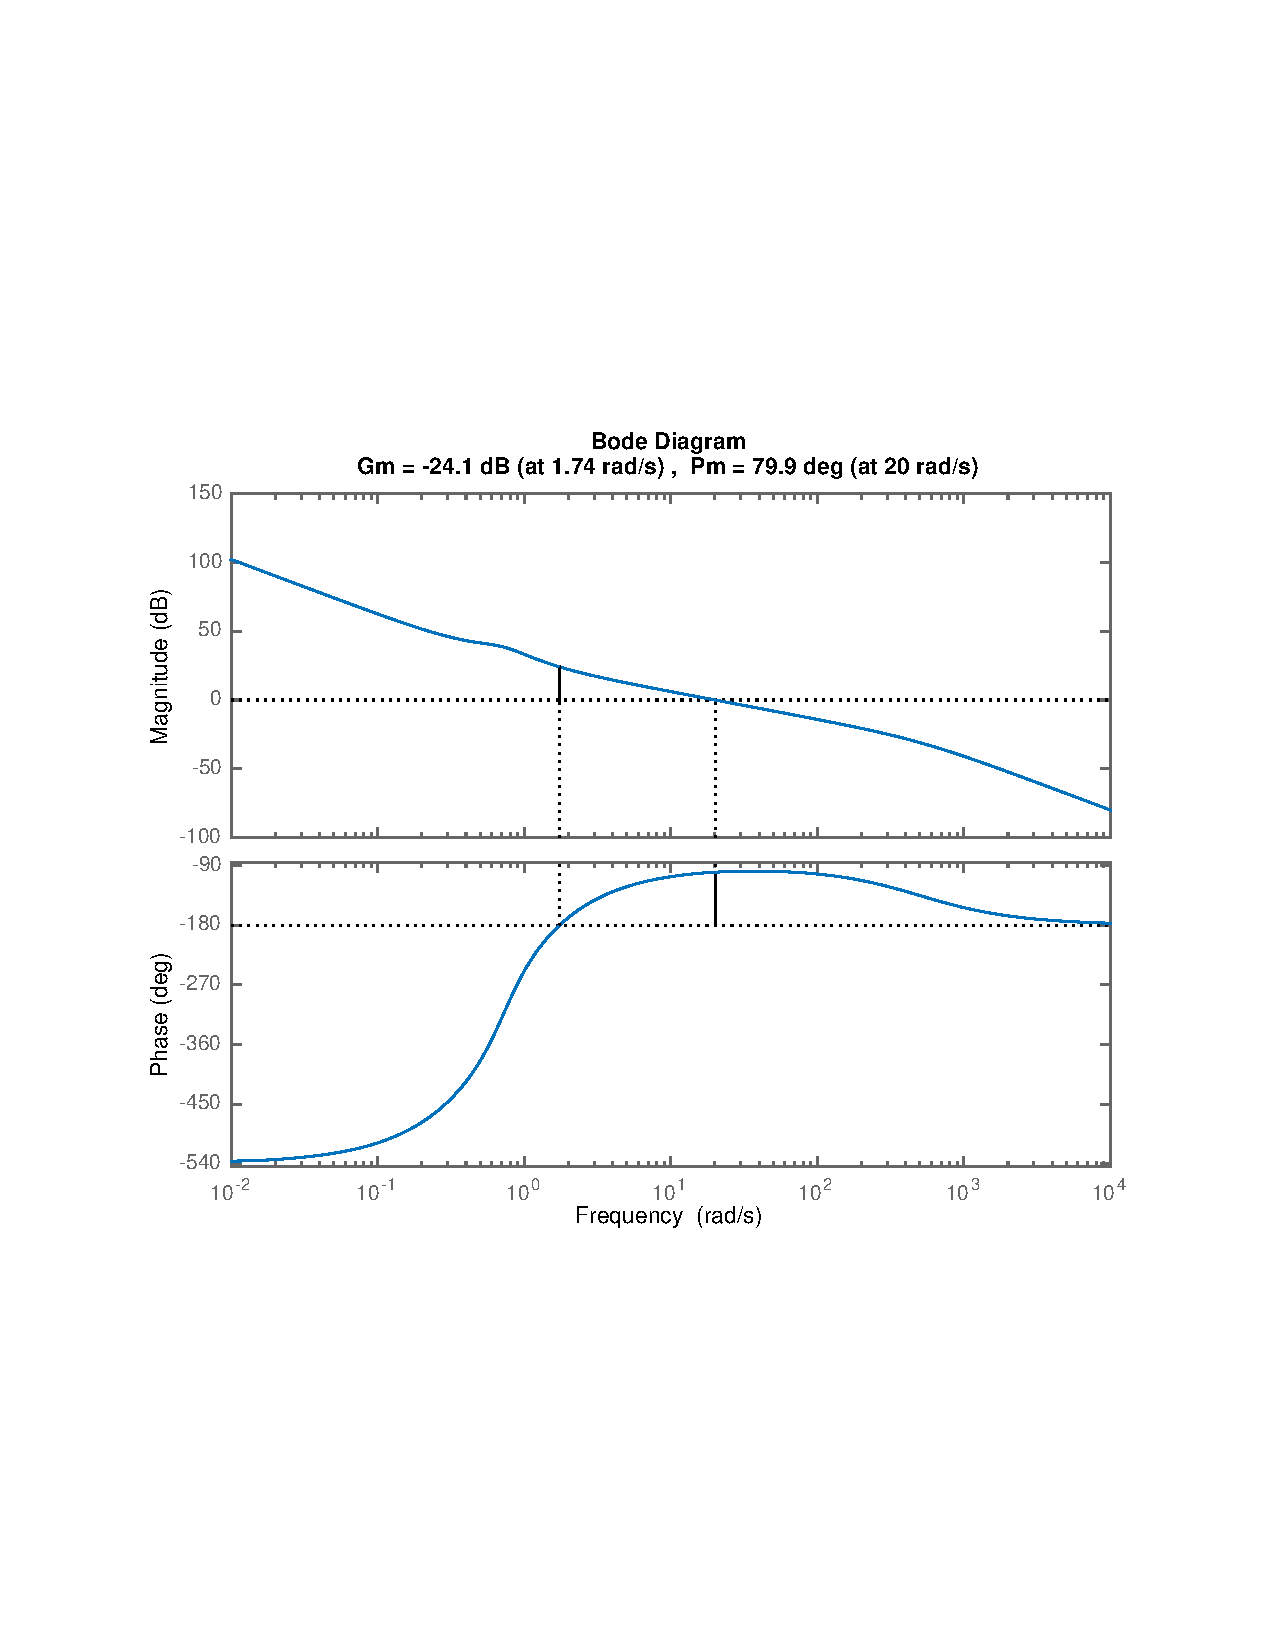
\includegraphics[width=1\textwidth]{figures/compensated_open_loop_bode}
\caption{Compensated Open Loop Bode Diagram}
% \label{}
\end{center}
\end{figure}

\begin{figure}[h]
\begin{center}
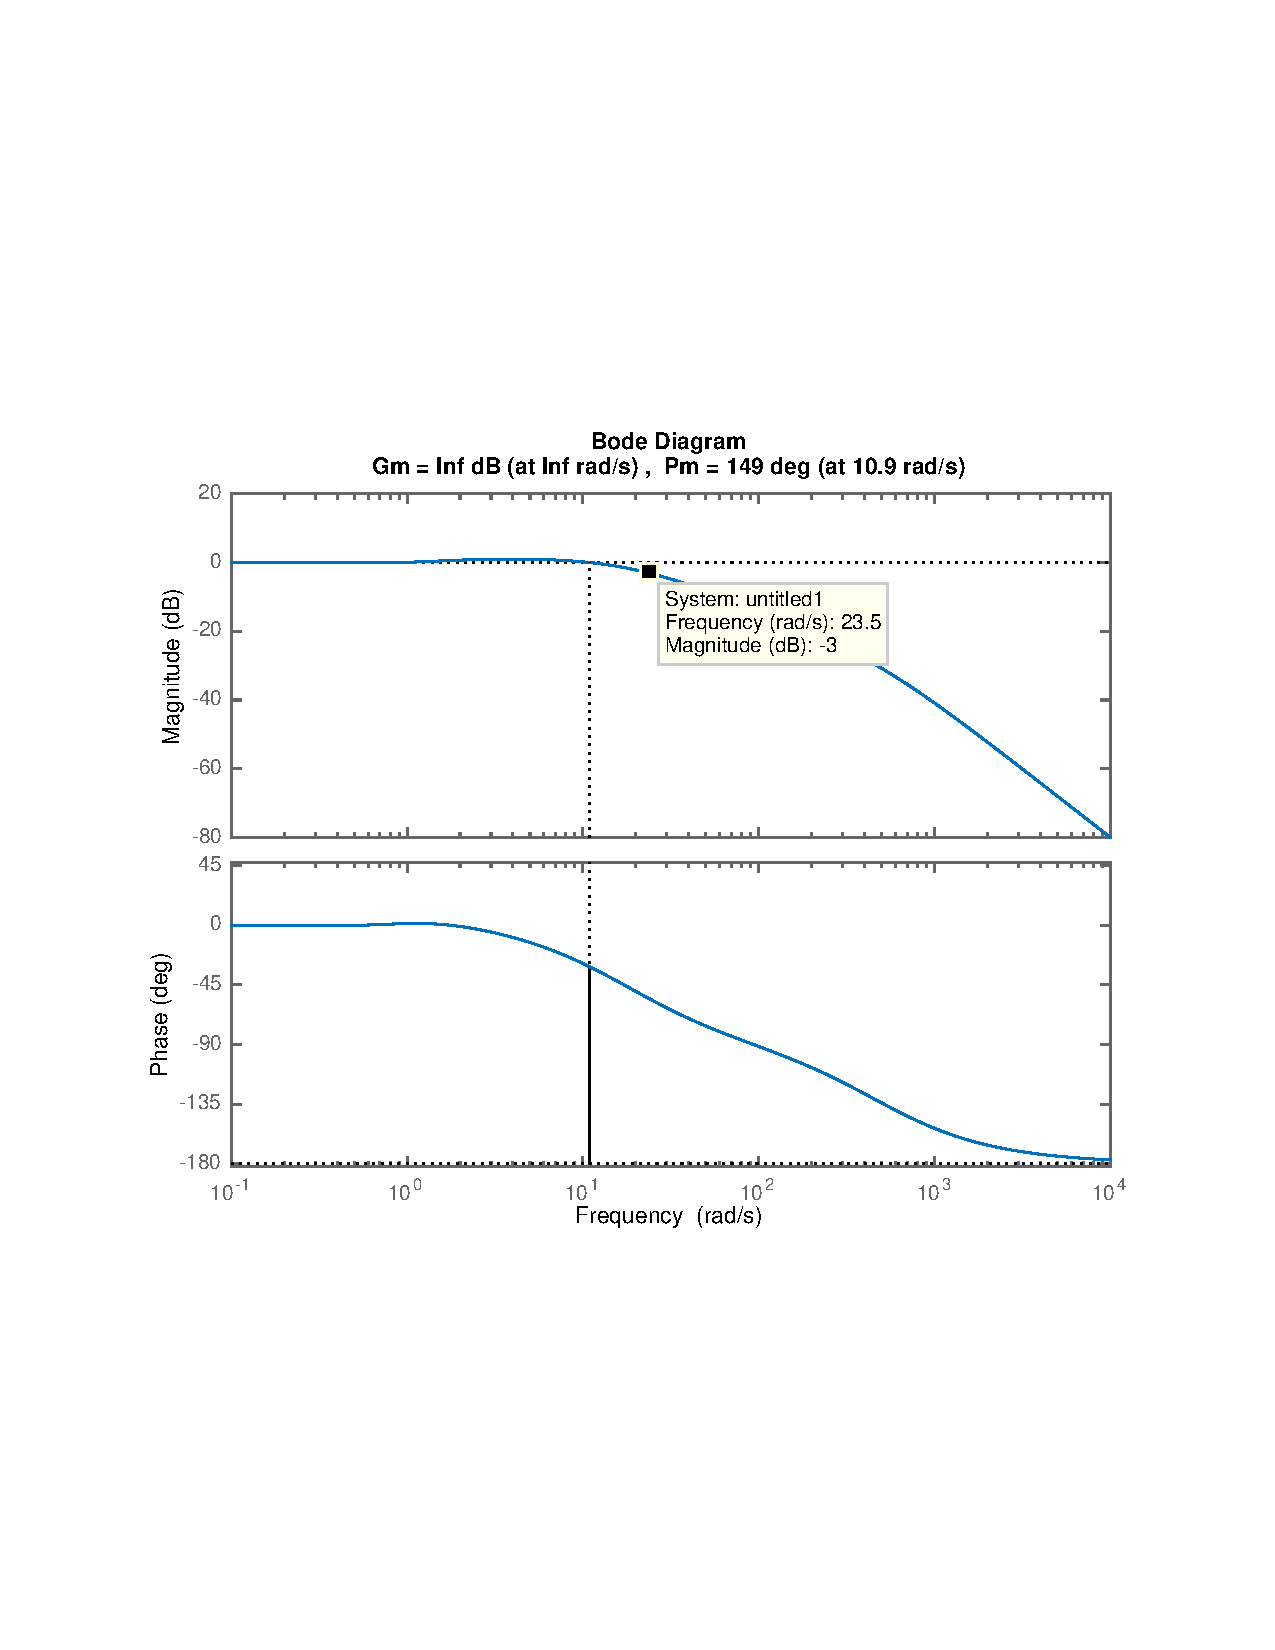
\includegraphics[width=1\textwidth]{figures/compensated_close_loop_bode}
\caption{Compensated Closed Loop Bode Diagram}
% \label{}
\end{center}
\end{figure}

\begin{figure}[h]
\begin{center}
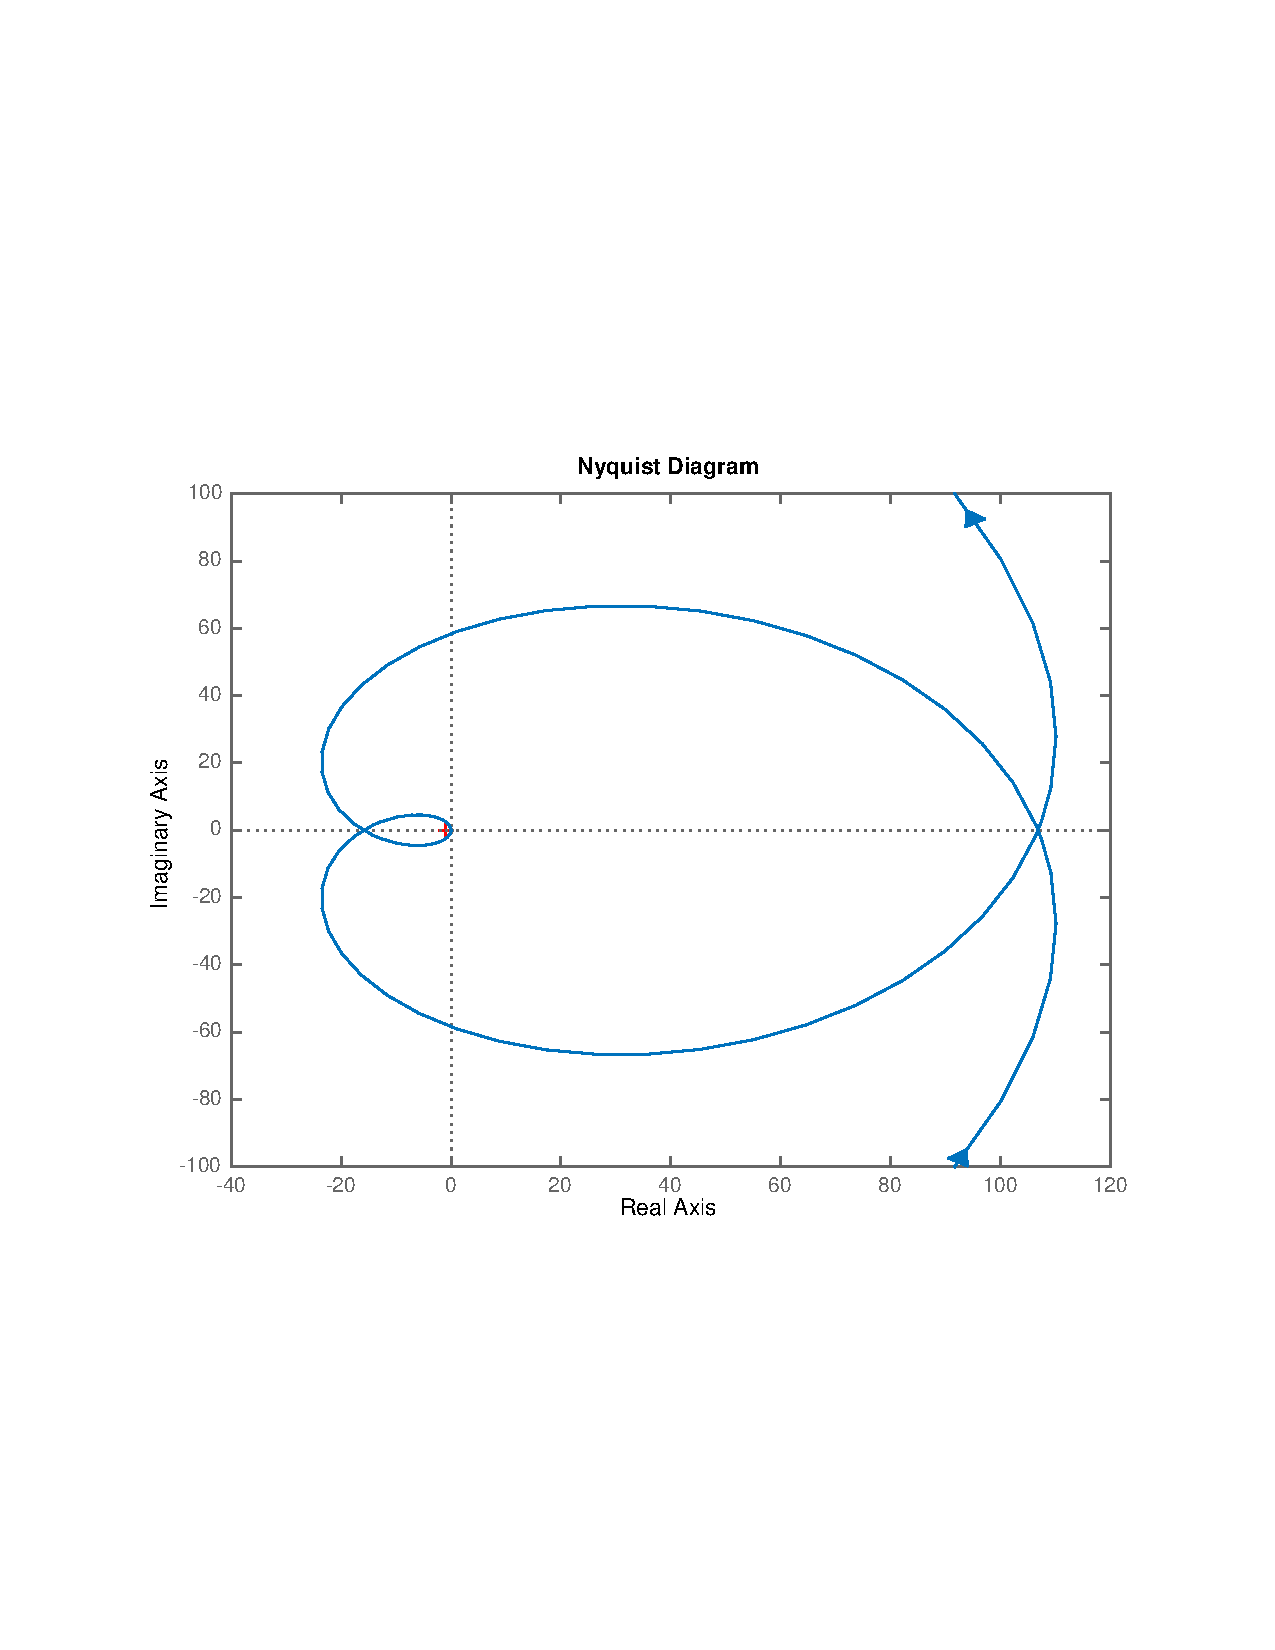
\includegraphics[width=1\textwidth]{figures/nyquist}
\caption{Nyquist Diagram}
% \label{}
\end{center}
\end{figure}

\clearpage
\section{Simulink Diagram and Step Response}
\begin{figure}[h]
\begin{center}
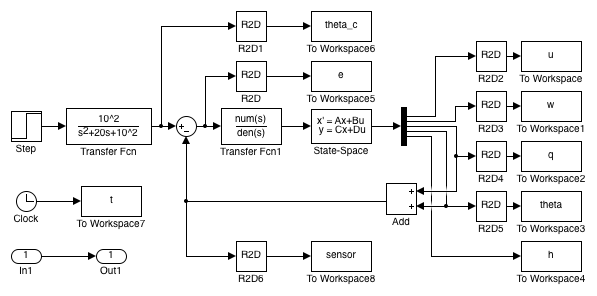
\includegraphics[width=1\textwidth]{figures/simulink}
\caption{Simulink Diagram}
% \label{}
\end{center}
\end{figure}

\begin{figure}[h]
\begin{center}
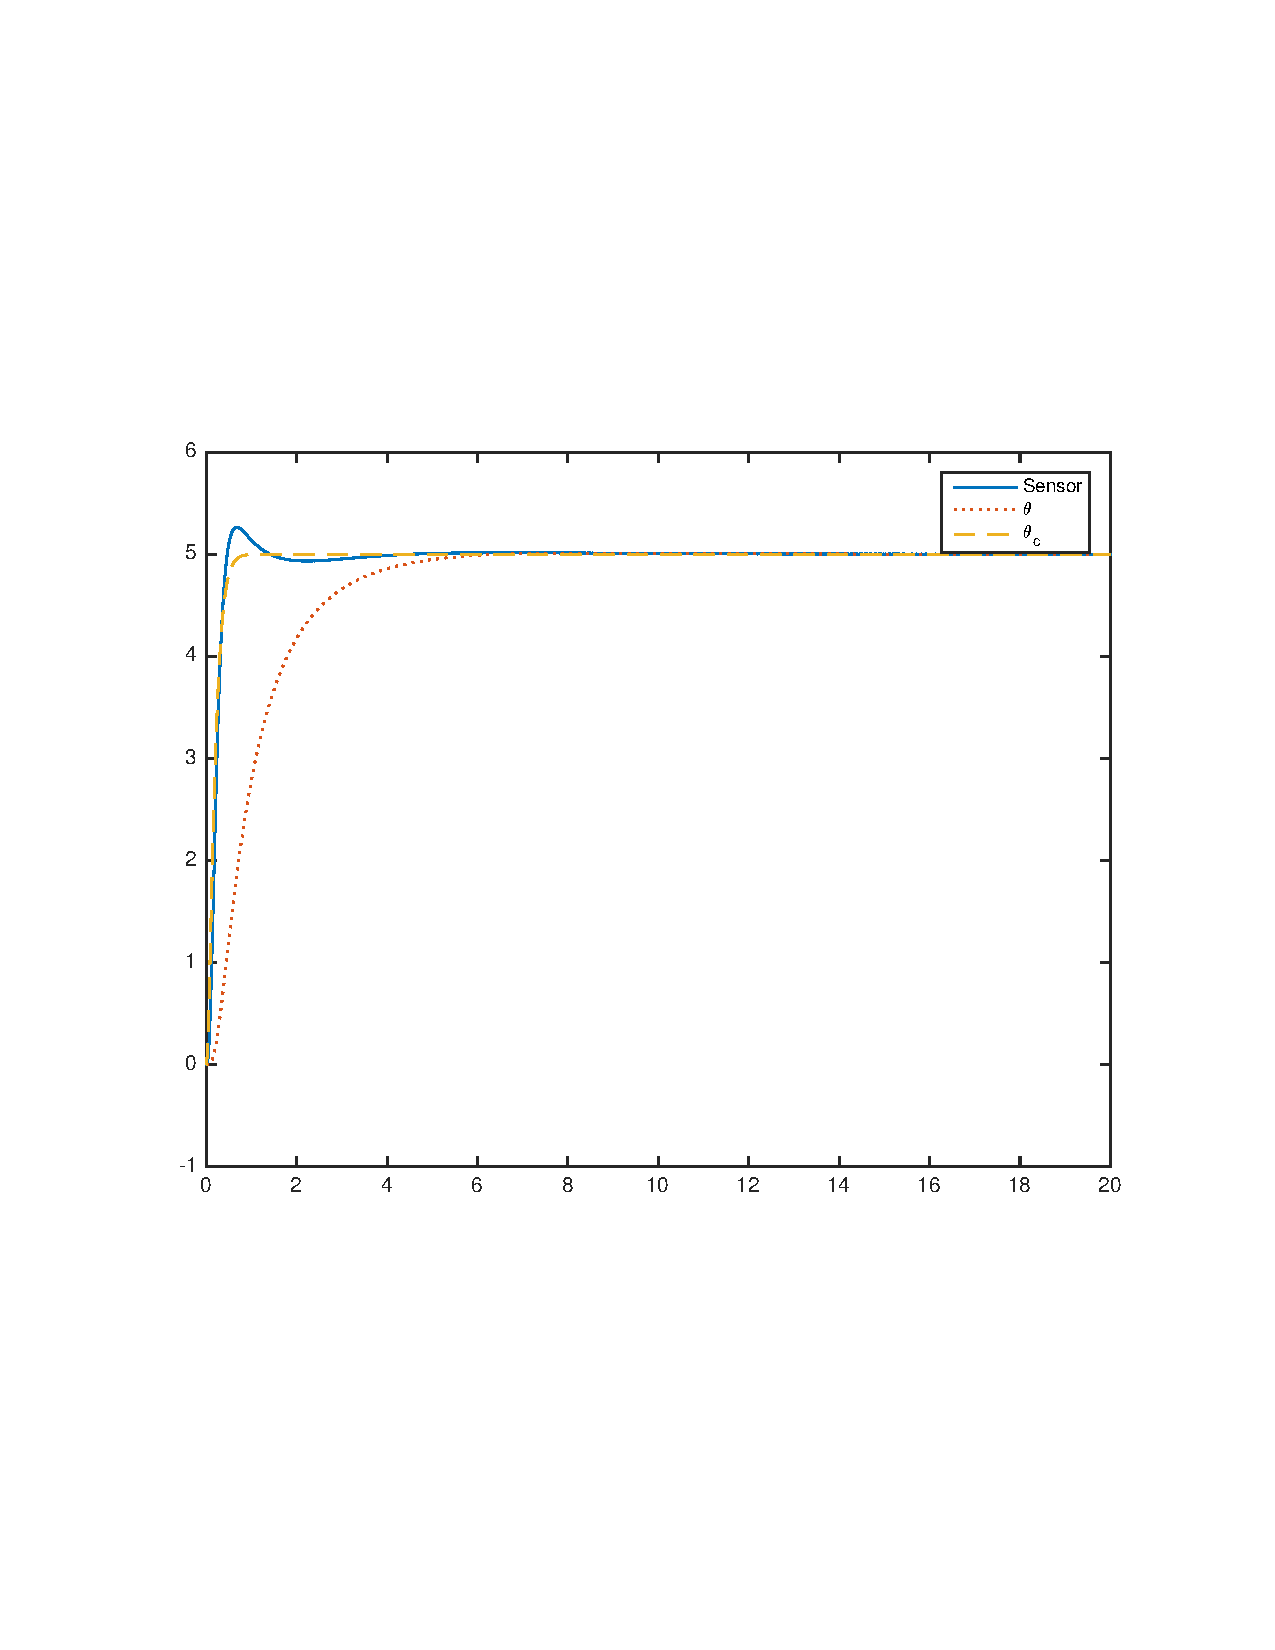
\includegraphics[width=1\textwidth]{figures/sensor}
% 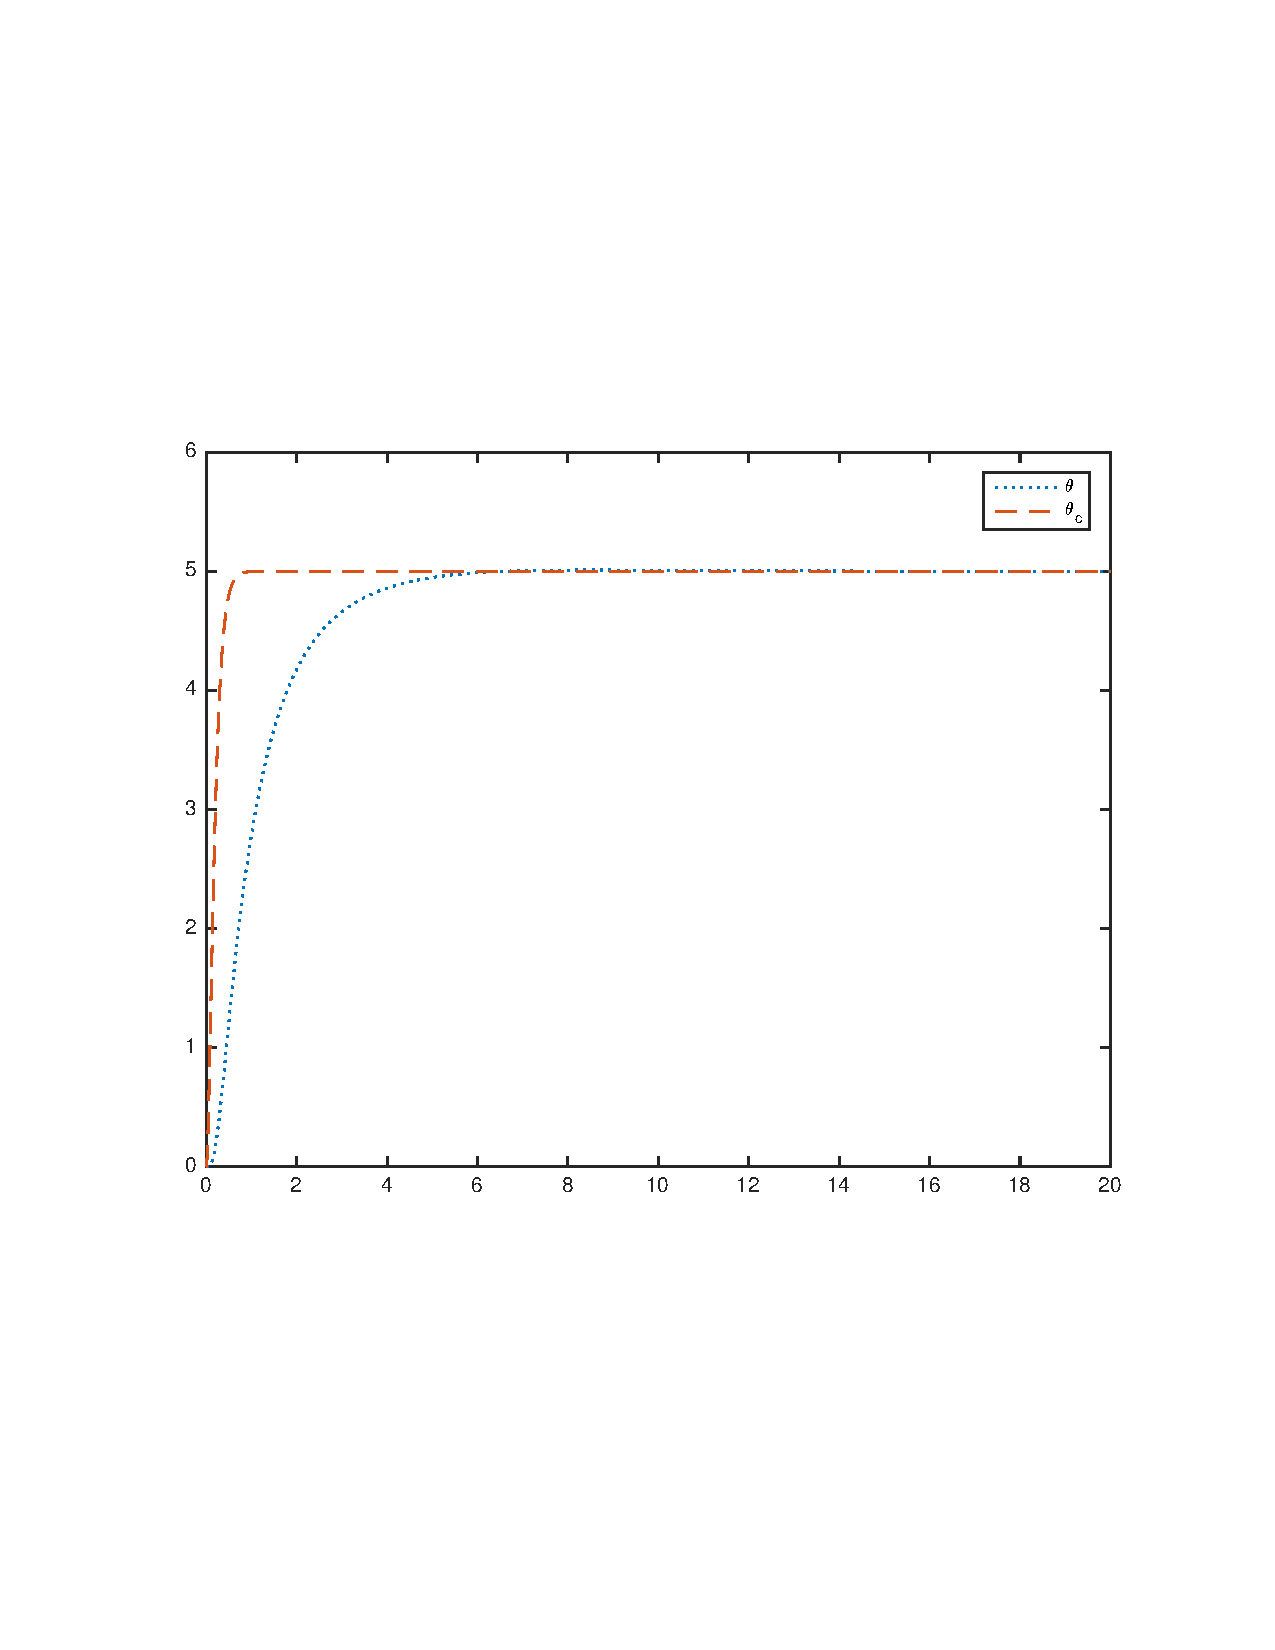
\includegraphics[width=1\textwidth]{figures/theta}
\caption{Step Response}
% \label{}
\end{center}
\end{figure}

% \begin{figure}[h]
% \begin{center}
% 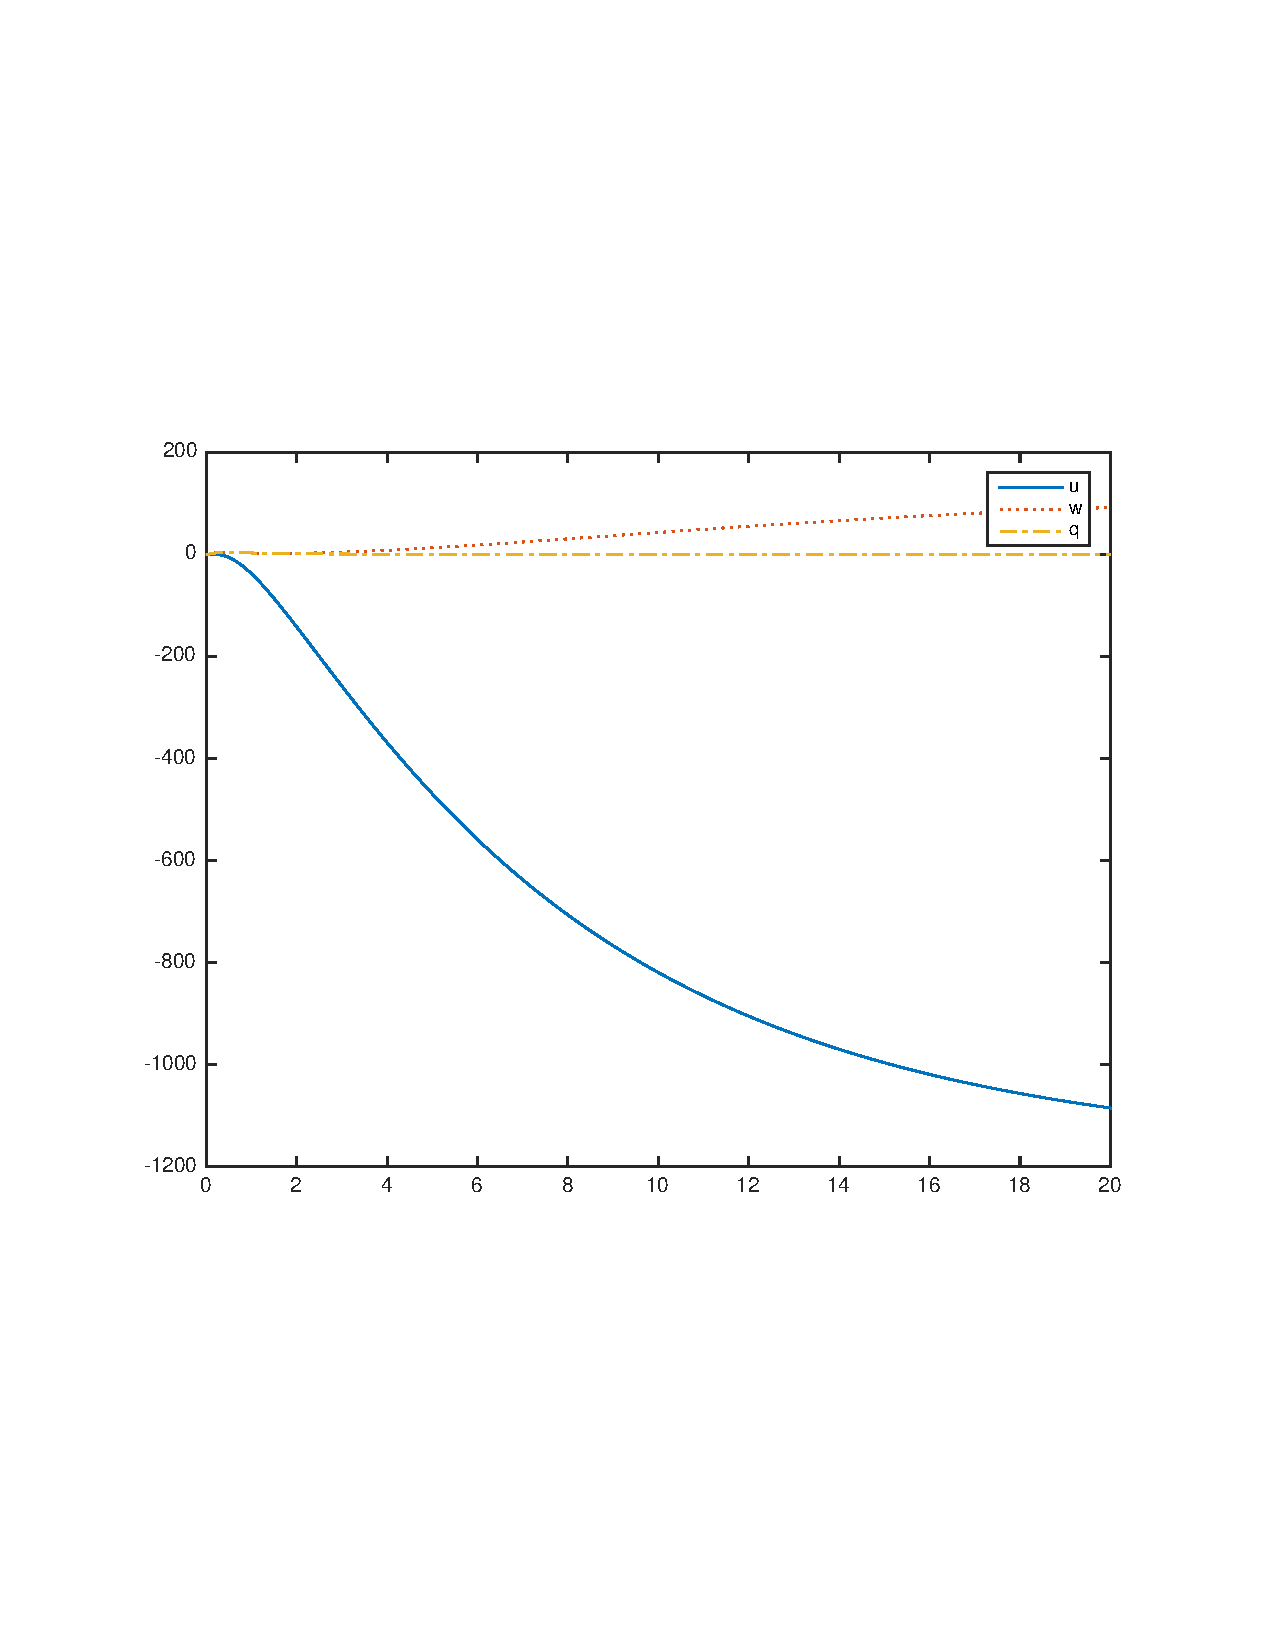
\includegraphics[width=1\textwidth]{figures/uwq}
% \caption{Step Response}
% % \label{}
% \end{center}
% \end{figure}

% \begin{figure}[h]
% \begin{center}
% 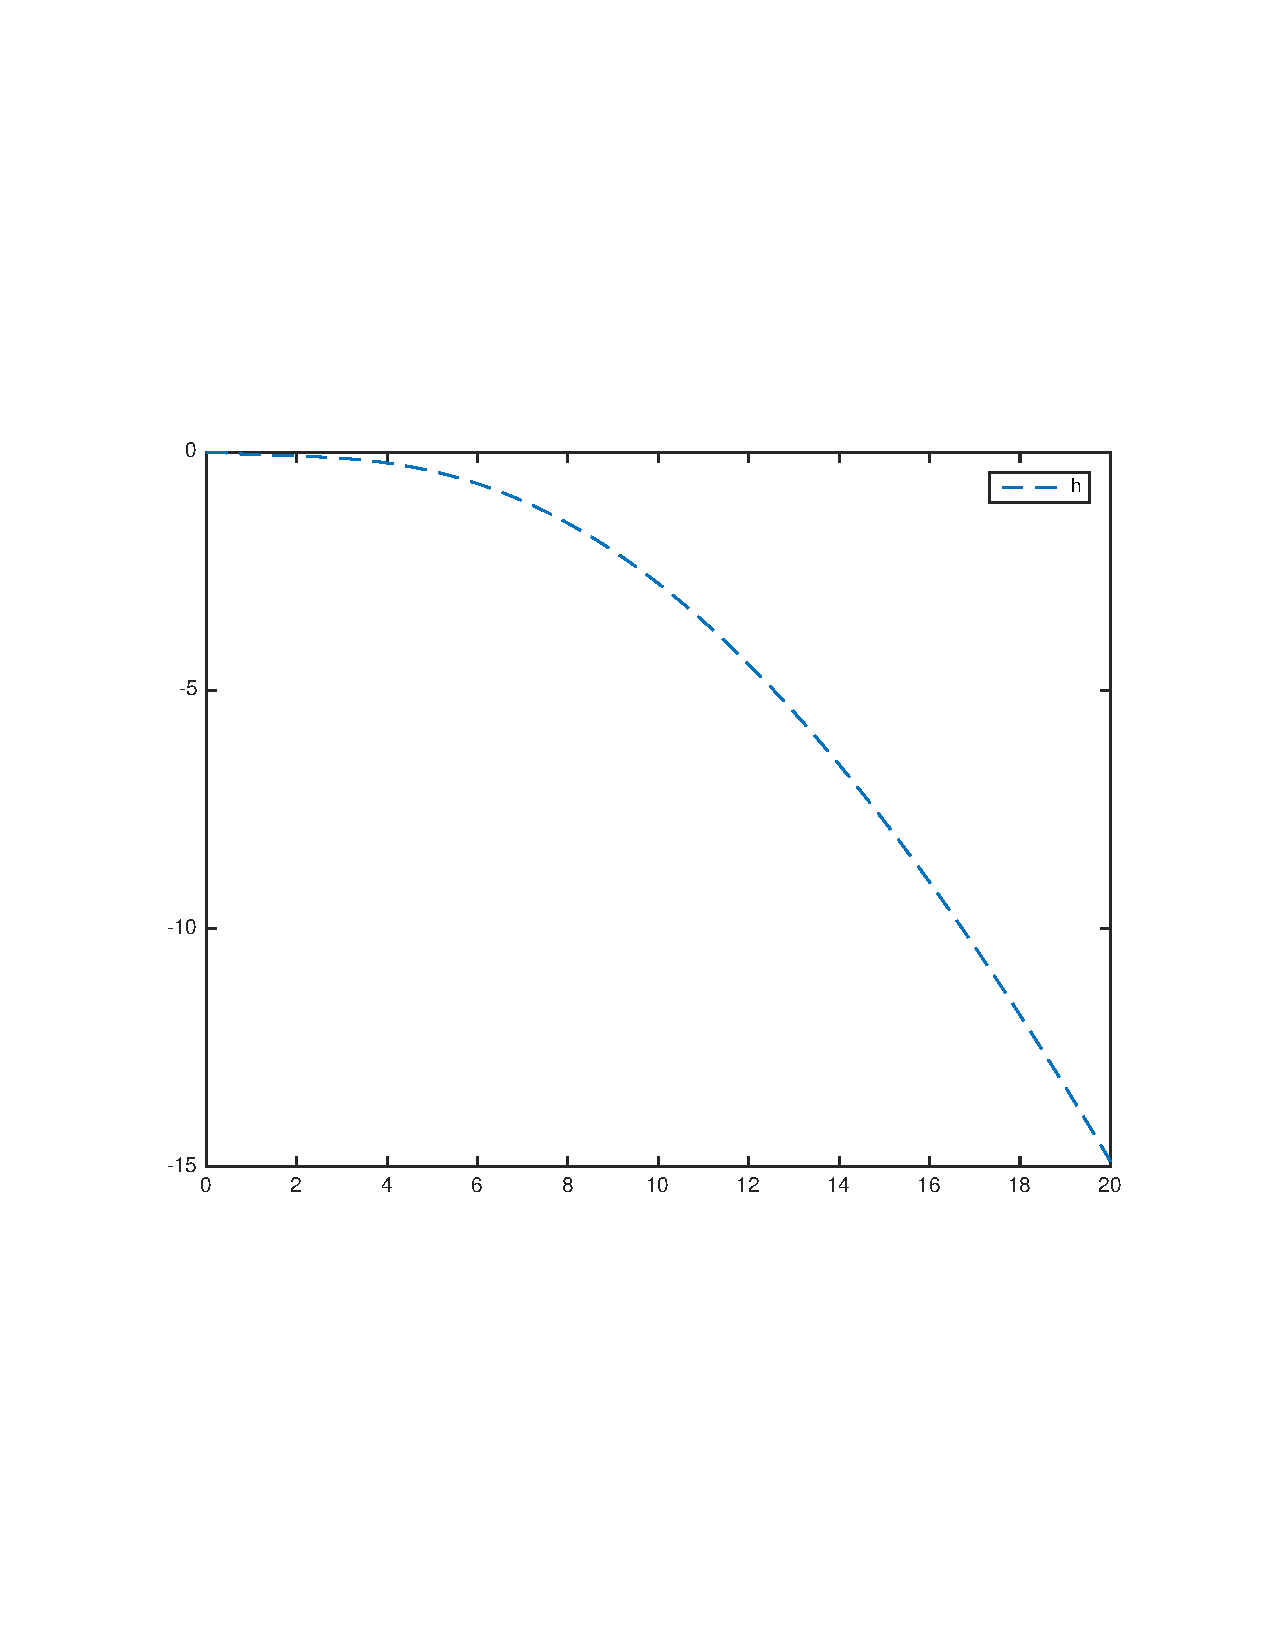
\includegraphics[width=1\textwidth]{figures/h}
% \caption{Step Response}
% % \label{}
% \end{center}
% \end{figure}

\end{document}
